% !TEX TS-program = pdflatex
% !TEX encoding = UTF-8 Unicode

% This is a simple template for a LaTeX document using the "article" class.
% See "book", "report", "letter" for other types of document.

\documentclass[11pt]{article} % use larger type; default would be 10pt

\usepackage[utf8]{inputenc} % set input encoding (not needed with XeLaTeX)

%%% Examples of Article customizations
% These packages are optional, depending whether you want the features they provide.
% See the LaTeX Companion or other references for full information.

%%% PAGE DIMENSIONS
\usepackage{geometry} % to change the page dimensions
\geometry{letterpaper} % a4paper or letterpaper (US) or a5paper or....
% \geometry{margin=2in} % for example, change the margins to 2 inches all round
% \geometry{landscape} % set up the page for landscape
%   read geometry.pdf for detailed page layout information

\usepackage{graphicx} % support the \includegraphics command and options

% \usepackage[parfill]{parskip} % Activate to begin paragraphs with an empty line rather than an indent

%%% PACKAGES
\usepackage{booktabs} % for much better looking tables
\usepackage{array} % for better arrays (eg matrices) in maths
\usepackage{paralist} % very flexible & customisable lists (eg. enumerate/itemize, etc.)
\usepackage{verbatim} % adds environment for commenting out blocks of text & for better verbatim
\usepackage{subfig} % make it possible to include more than one captioned figure/table in a single float
% These packages are all incorporated in the memoir class to one degree or another...

%%% HEADERS & FOOTERS
\usepackage{fancyhdr} % This should be set AFTER setting up the page geometry
\pagestyle{fancy} % options: empty , plain , fancy
\renewcommand{\headrulewidth}{0pt} % customise the layout...
\lhead{}\chead{}\rhead{}
\lfoot{}\cfoot{\thepage}\rfoot{}

%%% SECTION TITLE APPEARANCE
\usepackage{sectsty}
\allsectionsfont{\sffamily\mdseries\upshape} % (See the fntguide.pdf for font help)
% (This matches ConTeXt defaults)

%%% ToC (table of contents) APPEARANCE
\usepackage[nottoc,notlof,notlot]{tocbibind} % Put the bibliography in the ToC
\usepackage[titles,subfigure]{tocloft} % Alter the style of the Table of Contents
\renewcommand{\cftsecfont}{\rmfamily\mdseries\upshape}
\renewcommand{\cftsecpagefont}{\rmfamily\mdseries\upshape} % No bold!

%%% END Article customizations

%%% The "real" document content comes below...

\title{Automatic Model Calibration with Expert Knowledge}
\author{Jonathan Quebbeman, Shaun Carny, Gerald Day, John Park, Paul Micheletty}
%\date{} % Activate to display a given date or no date (if empty),
         % otherwise the current date is printed 

\begin{document}
\maketitle

\section*{Abstract}
Automatic model calibration using multiple objective algorithms has been in practice for decades, but several challenges include the development of pareto optimal solution sets with no physical meaning, inconsistent parameter convergence between trials, and increased parameter variance in the non-dominated population. Large sets of parameters can lead to \textit{compensatory calibration} with similar fitness but widely varied solution sets. To help guide the multi-objective evolutionary algorithm solution process, expert knownledge can be infused into an objective function leading to pareto solutions adhering to physically meaningful ranges, maintaining relationships between parameters, and creating increased regional consistency. This approach was applied to a case-study for calibrating the Animas River basin in Colorado using a the Research Distributed Hydrologic model and the Sacramento Soil Moisture Accounting and Snow-17 algorithms using the NSGA-II evolutionary algorithm. As a result of this process, fitness equal to or exceeding manual calibration was achieved, in addition to the development of realistic parameter set solutions.

\section{Introduction}

Genetic algorithms can be used for automatic model calibration using multiple objectives, which leads to a population of non-dominated solutions. Although the fitness of these solutions may be acceptable for each of the objectives, the corresponding parameter sets may not be physically realistic or meaningful. Manual review of the solutions by experts or third-parties may question the models given parameters on the extremes of acceptable ranges, or values may be contradicting each other. 

This can occur in over-determined problems with one parameter compensating for another, otherwise known as \textit{compensatory calibration}. Further, this creates population solutiions with increased variance. Since genetic algorithms include random perturbations, parameter convergence may occur in different regions with another independent trial if a random seed is not fixed. With multiple basins calibrated over a region, the increased diversity of solutions can create problems with parameter regionalization\cite{Steinschneider2015}.

These are not challenges when using a manual calibration process where the expert can utilize experience to retain expected ranges of parameters and maintain a regional consistency in the manual process. For regions with a large number of basins to be calibrated, or if the data is regularly updated leading to new calibrations, the manual process may not be feasible or cost-effective. Genetic algorithms are efficient 

\subsection{A subsection}



\section{Incorporation of Expert Knowledge}

$Fitness=f(Obs\:Q,\: Model\:Q,\: Parameter\: Set)$

\section{Case Study: Animas River Basin}
The Animas River Basin is a widely studied and monitored basin in the mountains of Colorado, USA, and is critically important for spring snow melt and water supply. Development of reliable estimates of yield from basins in this region is critical in support of basin water management. As part of a larger study, a Research Distributed Hydrologic Model (RDHM) model\cite{Koren2004} was developed using the Sacramento Soil Moisture Accounting (SAC-SMA) model [National Weather Service], and snow accumulation and ablation was estimated with Snow-17 \cite{Anderson2006}.

A Non-Dominated Sorting Genetic Algorithm (NSGA-II) \cite{Deb2002} was wrapped around the hydrologic model using three objective fitness functions. Each objective should be \textit{minimized}, therefore negative values were uses where needed.

\subsection{Fitness Functions}
\paragraph{Fitness-1: Negative Kling-Gupta} The Kling-Gupta\cite{Gupta2009} fitness includes three components of bias, variance, and correlation, described as follows.

$Kling-Gupta=1-\sqrt{(R^2-1.)^2+(Var-1)^2+(MeanBias-1)^2)}$

where,

$MeanBias=\mu_{model}/\mu_{obs}$

$Var= (\sigma_{model}/\mu_{model})/(\sigma_{obs}/\mu_{obs})$

$R^2=Correlation(Obs,Mod)$

The \emph{negative} Kling-Gupta value is used in the NSGA-II algorithm.

\paragraph{Fitness-2: Monthly Volume Bias} This estimates the mean difference between total monthly observed and calculated volumes and selects the maximum mean monthly difference. 

$max\{|mean_{month}(Vol_{obs}-Vol_{model})|\}$

\paragraph{Fitness-3: Expert Knowledge} The expert knowledge oibjective is the sum of a collection of penalties based solely on the parameters of the given solution. With no parameter violations, the objective would be perfect and have a score of $0$. 

$\sum_{i=1}^M ParameterPenalty_i + \sum_{j=1}^N RelationPenalty_i$

Individual parameter penalty functions can be sharp, linearly gradated, or both. A sample figure of different parameter penalty functions is shown in Figure-\ref{Param_Penalty}. Not for these examples, each parameter includes a region of no-penalty, a region on the higher end of values with a slowly gradated increase in penalty (the not-preferred zone), and a region on the lower end of relatively sudden increases in penalty. 

Penalties are also used for the relationship between certain parameter sets as shown in Figure-\ref{Joint_Penalty}. In these cases, experts expressed that one variable should not be above a threshold if the other is below some level. These joint penalty functions are expressions of their regional knowledge - alternative forms are certainly possible, and could include non-linear relationships if users are aware of these functions and are able to express them mathematically.

\subsection{Testing Approach}
As additional objective functions are added, the non-dominated set may adversely affect other solution spaces with reduced fitness. Leaving the first two fitness functions in-place, would the addition of the expert knowledge objective (Fitness-3) result in degraded performance for Fitness-1 and Fitness-2? Further, can it be demonstrated that the algorithm results in decreased variance between trials, and decreased variance between solutions in a single pareto set?

Two parallel and identical model calibration trials were developed, with the exception of one trial including the third fitness expert knowledge fitness function (i.e. 2-Objective vs. 3-Objective). 

A second test was developed using the same model configurations, which involved the repeated optimization process in 35 independent trials. This test is used to compare the ability for consistent convergence of parameters in certain ranges, relative to the 2-Objective model without expert knowledge.

\subsection{Results}
Individual members in the non-dominated pareto front produce very similar fitness in the hydrographs - Figure-\ref{Hydrographs} shows a selection of hydrographs from five different members compared to both the observations and the manually calibrated values. Kling-Gupta values and monthly biases are very similar between all non-dominated solutions and additional pareto solution selection metrics would be needed to choose a single member (e.g. regionalization, expert preference or weighting methods for objectives, or a new post-processing objective). These figures show a successful use of the algorithm to develop calibrated parameters.

When compraing the 3-Objective to the 2-Objective approach, a similar level of fitness for the first two objectives is achievable. Figure-\ref{Objective_Compare} shows a) all solution member from all fronts, and b) the non-dominated solutions from both approaches. Although the shape of the field appears different when extending from 2 to 3-dimensions, the range on the non-dominated sets are very similar. This same information can also be viewed as histograms and is shown in Figure-\ref{Fitness_Compare}.

This process was repeated for 35 independent trials using the 2 or 3-Objective approaches. As shown in Figure-\ref{Reduced_Variance} for the parameter $UADJ$, there is increased variance across the pareto front for each individual trial when expert knowledge is not incorporated. Further, the range of results extends across the entire acceptable space with each trial converging in different regions. Alternatively with the inclusion of 3-Objectives and the expert knowledge, the individiual trial variance is reduced, and the intra-trial variance is also reduced creating consistency between independent trials. The values destimated are within acceptable and believable ranges.

Although $UADJ$ demonstrated decreased variance, in some cases the variance increased.

\section{Conclusions}

Increased variance in certain parameters.

Recognize different regions and models will require different expert elicitation and development of penalties.


\bibliographystyle{plain}
\bibliography{Riverside}

\begin{figure}
\centering
\noindent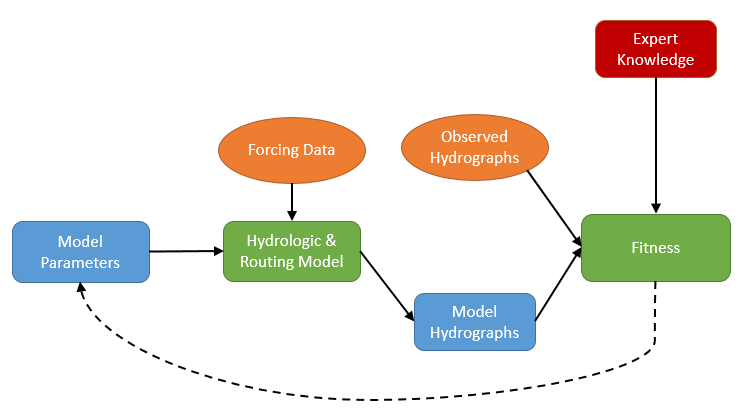
\includegraphics[scale=.7]{./Figures/Process.png} 
\caption{Inclusion of Expert Knowledge in genetic algorithm}
\label{Process}
\end{figure}

\begin{figure}
\centering
\noindent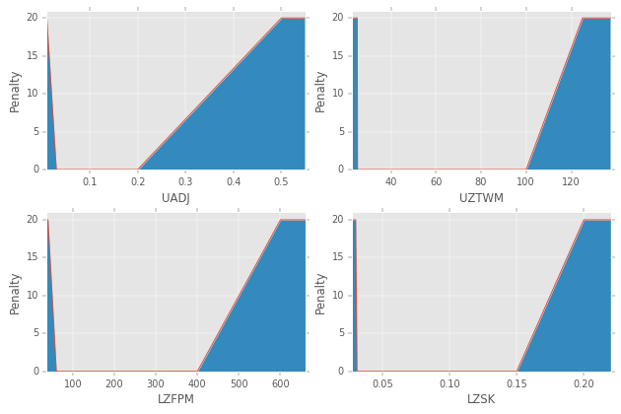
\includegraphics[scale=.7]{./Figures/Parameter_Penalties.png} 
\caption{Examples of parameter ranges and shoulder penalties}
\label{Param_Penalty}
\end{figure}

\begin{figure}
\centering
\noindent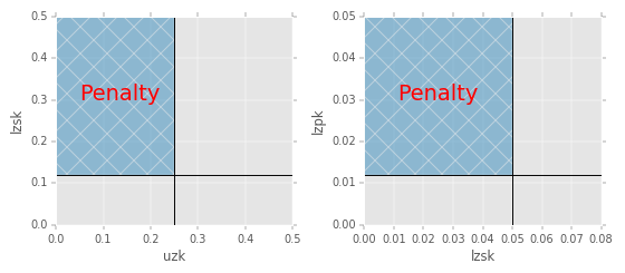
\includegraphics[scale=.7]{./Figures/Joint_Parameter_Penalties.png} 
\caption{Example of correlated parameter penalties (LZSK and UZK, LZPK and LZSK)}
\label{Joint_Penalty}
\end{figure}

\begin{figure}
\centering
\noindent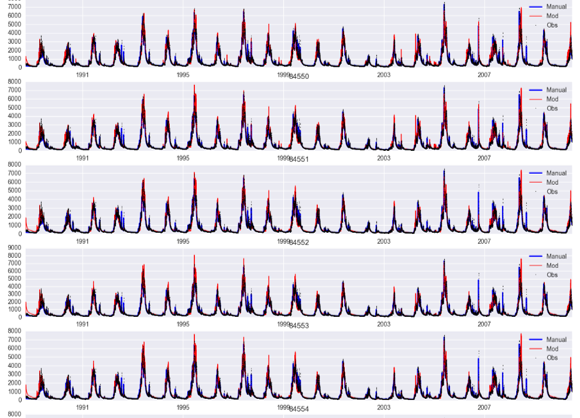
\includegraphics[scale=1]{./Figures/Hydrographs.png} 
\caption{Comparison of calibrated hydrographs for five selections on the Pareto front against manual solution and observed data}
\label{Hydrographs}
\end{figure}

\begin{figure}
\centering
\noindent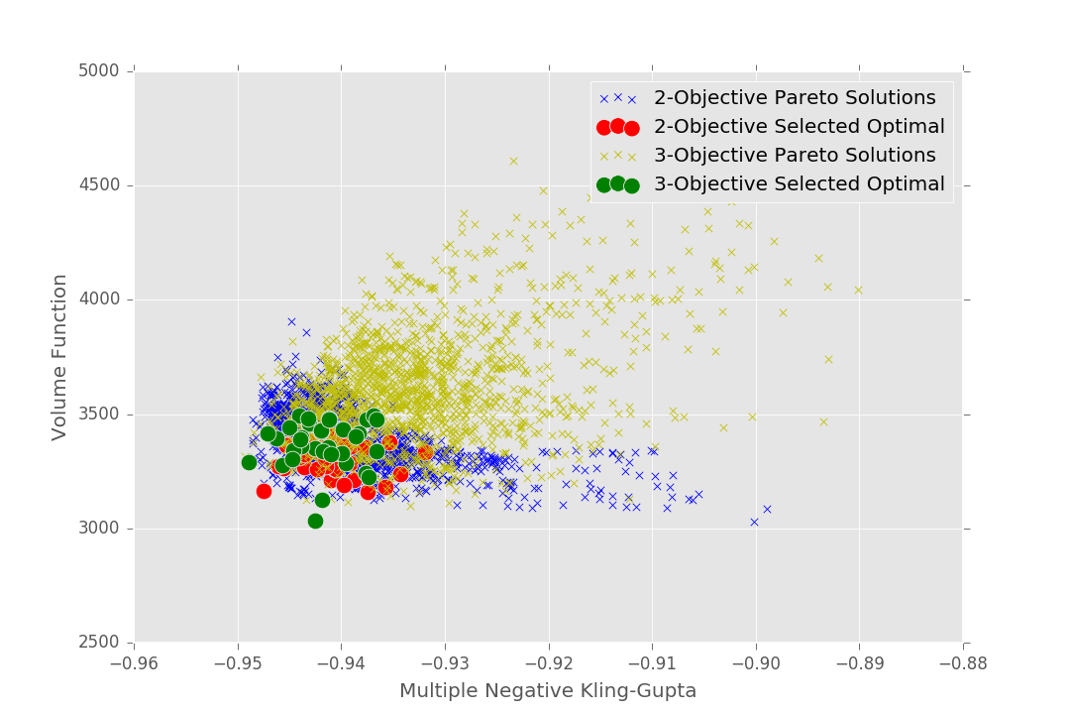
\includegraphics[scale=.7]{./Figures/Objective_Compare.png} 
\caption{Population and Non-dominated solution objectives for both 2-objective and 3-objective approaches (inclusion of expert knowledge)}
\label{Objective_Compare}
\end{figure}

\begin{figure}
\centering
\noindent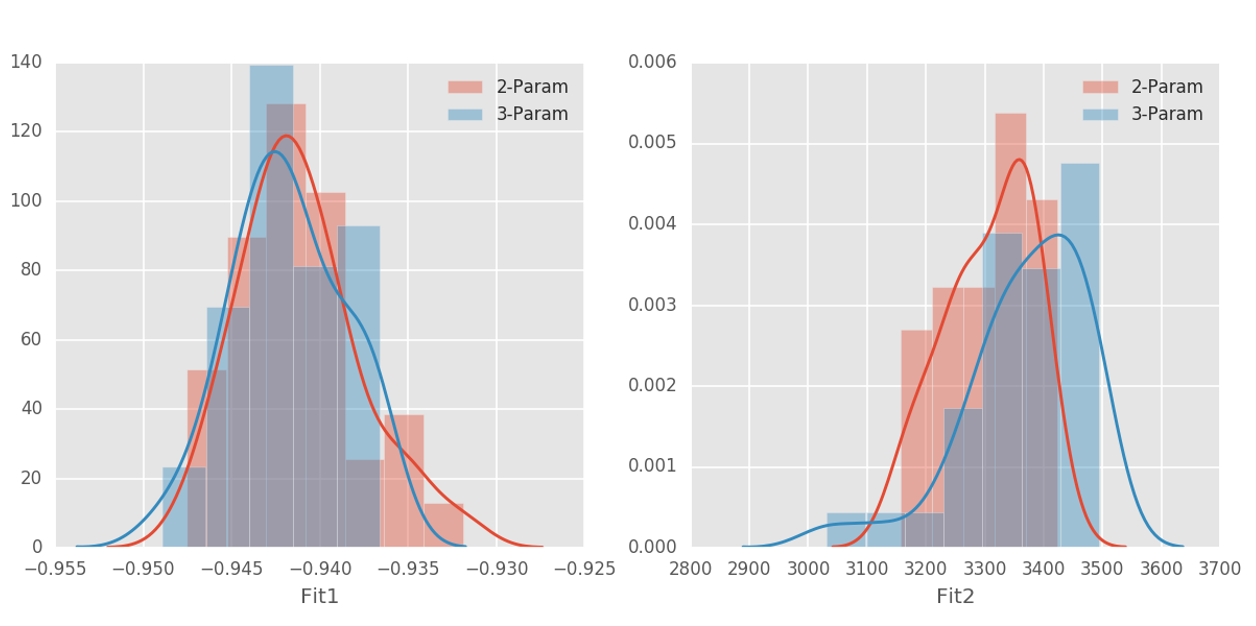
\includegraphics[scale=.6]{./Figures/Fitness_Compare.png} 
%\caption[Hourly Optimal Stomatal Responses with Original Observed Data (June 14, 1983)]{LONG CAPTION}
\caption{Comparison of first two fitness functions using either a) only those two objectives, or b) the additional parameter constraint objective.}
\label{Fitness_Compare}
\end{figure}

\begin{figure}
\centering
\noindent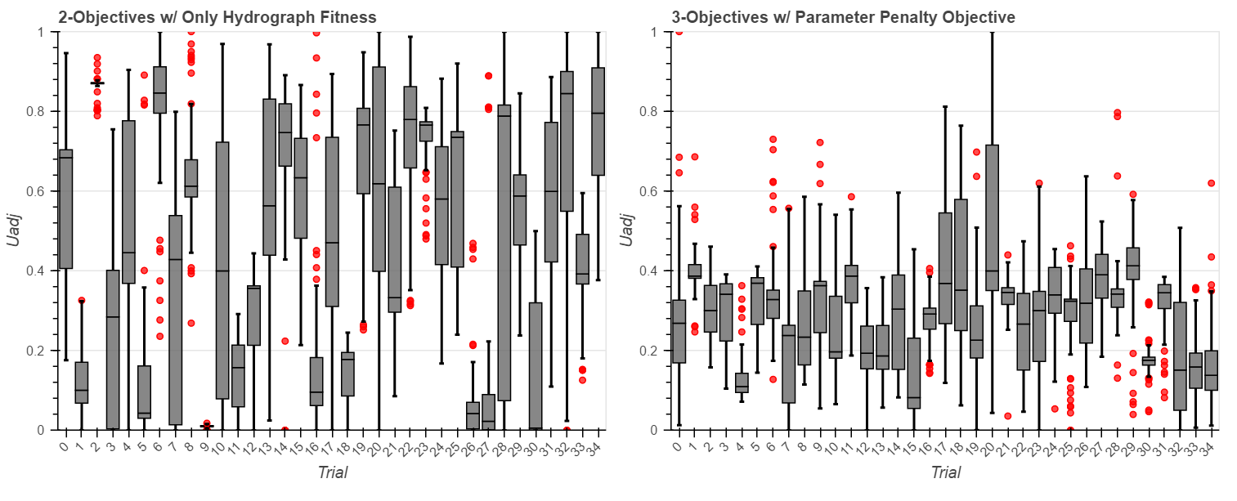
\includegraphics[scale=.5]{./Figures/Reduced_Variance_UADJ.png} 
\caption{Inter-trial variance from independent calibration runs improving consistency and reproducibility}
\label{Reduced_Variance}
\end{figure}




\end{document}
